\documentclass[12pt]{report}
\usepackage[utf8]{inputenc}
\usepackage[T1]{fontenc}
\usepackage[a4paper, left=2.4cm, right=2.4cm, top=2cm, bottom=2cm, nomarginpar]{geometry}
\usepackage{amsmath, algorithm, pgfplots, pgf, pdfpages, amsfonts, amssymb, stmaryrd, enumitem,graphicx, algpseudocode, setspace, listings, courier, color, caption, centernot, hyperref, lstautogobble, zi4, mathtools, lmodern, colortbl, array, multicol, fancyhdr, lastpage, svg}
\usepackage{booktabs}
\hypersetup{
    pdftitle={CE204_FP1_G6},
    pdftoolbar=true,        % show Acrobat’s toolbar?
    pdfmenubar=true,        % show Acrobat’s menu?
    pdfauthor={Muhammet Yağcıoğlu},
    pdfsubject={CE204_FP_RPs},
    pdfcreator={Muhammet Yağcıoğlu},   % creator of the document
    pdfproducer={Muhammet Yağcıoğlu}, % producer of the document
    colorlinks,
    linkcolor={black},
    citecolor={black},
    urlcolor={blue!80!black}
}
\usepackage[noblocks]{authblk}
\usepackage[version=4]{mhchem}
\usepackage[export]{adjustbox}
\usepackage{eso-pic} % Required for absolute positioning
\graphicspath{ {./images/} }
\usetikzlibrary{patterns}
\usepackage{tikz-3dplot}
\usepackage[version=4]{mhchem}
\usepackage[export]{adjustbox}
\usepgfplotslibrary{groupplots}
\usepackage{xcolor}
\usepackage[absolute,overlay]{textpos}
\usepackage{ragged2e}
\usepackage{xcolor}
\usepackage{amsthm}
\usepackage{tikz}




%----------compiler settings---------
\setlength{\parindent}{0pt}
\everymath{\displaystyle}
\onehalfspacing

%-----------colors----------
\pgfplotsset{compat=1.18}
\definecolor{bluekeywords}{rgb}{0.13, 0.13, 1}
\definecolor{greencomments}{rgb}{0, 0.5, 0}
\definecolor{redstrings}{rgb}{0.9, 0, 0}
\definecolor{graynumbers}{rgb}{0.5, 0.5, 0.5}
\definecolor{bronze}{rgb}{0.82, 0.41, 0.12}
\definecolor{crimson}{rgb}{0.86, 0.08, 0.24}
\definecolor{brown(web)}{rgb}{0.65, 0.16, 0.16}
\definecolor{darkspringgreen}{rgb}{0.16, 0.32, 0.75}
\definecolor{blue(ncs)}{rgb}{0.0, 0.53, 0.74}
\definecolor{amber}{rgb}{1.0, 0.49, 0.0}
\definecolor{cadmiumgreen}{rgb}{0.0, 0.42, 0.24}




%-------code frame-----------
\lstset{
    autogobble,
    columns=fullflexible,
    showspaces=false,
    showtabs=false,
    breaklines=true,
    showstringspaces=false,
    breakatwhitespace=true,
    escapeinside={(*@}{@*)},
    commentstyle=\color{greencomments},
    keywordstyle=\color{bluekeywords},
    stringstyle=\color{redstrings},
    numberstyle=\color{graynumbers},
    basicstyle=\ttfamily\footnotesize,
    frame=l,
    framesep=12pt,
    xleftmargin=12pt,
    tabsize=4,
    captionpos=b
}



\lstdefinelanguage{myMMA}{
keywords={SetDirectory, NotebookDirectory, Exp, IdentityMatrix, Eigenvalues, 
ListPlot, PlotRange, PlotStyle, Directive, PointSize, AspectRatio, Blue, Graphics, Line, 
Manipulate, Show, Sqrt, UniformDistribution, GammaDistribution, BetaDistribution, 
Nintegrate, For, DataRange, AxesLabel, PlotLabel, Transpose, Export, Plot, Append, Infinity},
keywordstyle=\color{black},
commentstyle=\color{gray}, 
identifierstyle=\color{blue},
sensitive=false,
comment=[l]{(*},
morecomment=[s]{/*}{*/},
morestring=[b]',
morestring=[b]"
}






%-----gauss declare---------
\pgfmathdeclarefunction{gauss}{2}{%
  \pgfmathparse{1/(#2*sqrt(2*pi)) * exp(-((x-#1)^2)/(2*#2^2))}%
}
\usetikzlibrary{arrows.meta, decorations.markings}
\pgfplotsset{compat=1.17}







%--------------page numbering------------
\fancyfoot[R]{page \thepage\ of \textcolor{bronze}{\pageref{LastPage}}}
\fancyhead[R]{Group 6}



%-------------qframe settings---------------

\usepackage[framemethod=TikZ]{mdframed}
\newmdenv[%
    skipabove=1em, % space above the frame
    skipbelow=1em, % space below the frame
    linewidth=1pt, % width of the frame lines
    linecolor=gray!80, % color of the frame lines
    backgroundcolor=gray!9, % background color inside the frame
    roundcorner=5pt, % radius of the rounded corners
    innerleftmargin=1em, % margin within the frame at the left
    innerrightmargin=1em, % margin within the frame at the right
    innertopmargin=0.5em, % margin within the frame at the top
    innerbottommargin=0.5em % margin within the frame at the bottom
]{qframe}

\newenvironment{q}
{
    \begin{qframe}
    \noindent\textit{\textbf{Problem Statement:}}
    \par\smallskip
}
{
    \end{qframe}
}





%-------------ANSWER TAG---------------
\newcommand{\AnswerTag}{\hfill 
\begin{tikzpicture} \fill[black] (0.35cm,0) -- (0,0.175cm) -- (0.35cm,0.35cm) -- cycle;\end{tikzpicture}}



%-------Theorem and another question frames----------
\newenvironment{theorem}{\begin{mdframed}\textbf{Theorem.}}{\end{mdframed}}

%usage: \begin{theorem}

\newenvironment{question}{\begin{mdframed}\textbf{Question.}}{\end{mdframed}}

%usage: %usage: \begin{question}
\fancyhead[L]{CE204 Engineering Surveying - Report of Field Practice 2}
\author{Muhammet Yağcıoğlu - 290204042}
\usepackage{hyperref} 

\begin{document}
\onecolumn
\thispagestyle{empty}
\begin{center}


\textbf{\fontsize{14}{\baselineskip}\selectfont İzmir Institute of Technology}


\textbf{\fontsize{14}{\baselineskip}\selectfont In collaboration with}


\textbf{\fontsize{14}{\baselineskip}\selectfont Department of Civil Engineering}

\bigskip

\includesvg[width=5cm]{Picture1.svg}

\bigskip

\textbf{\fontsize{15}{\baselineskip}\selectfont CE204 – ENGINEERING
SURVEYING}

\bigskip

\textbf{\fontsize{16}{\baselineskip}\selectfont 2023-2024 SPRING}

\bigskip

\bigskip



\textit{\textbf{\fontsize{14}{\baselineskip}\selectfont Field Practice – 2}}

\bigskip



\bigskip

\textbf{\fontsize{14}{\baselineskip}\selectfont Lecturer: Assoc. Prof. Volkan Emre UZ }

\bigskip

\textbf{\fontsize{14}{\baselineskip}\selectfont Group 6}

\bigskip

\textbf{\fontsize{14}{\baselineskip}\selectfont Team Leader: Melih Berke	KARAADAM}

\bigskip

Melih Berke	KARAADAM\\
Mert BAY\\
Mert BOSTANCI \\
Mevlüt Yağız KÜL\\
Muhammet YAĞCIOĞLU\\
Muhammet Taylan ARSLAN\\


\bigskip

\bigskip

\bigskip

{\today}
\end{center}

\clearpage




\thispagestyle{fancy}
\pagestyle{fancy}

\newpage
\begin{abstract}
The precision of conventional land surveying techniques for calculating the size of a pentagonal plot is tested in this field exercise.  We used height-based calculations, the cross technique, and direct linear measurement using a steel tape.  We used each method to compute the area many times. The accuracy of each technique was quantified by statistical analysis. Traditional surveying procedures provide accurate area calculations, according to the results. More investigation into combining these techniques with contemporary technology could lead to even more efficiencies and accuracy gains.
\end{abstract}
\tableofcontents
\newpage
\section*{Introduction}
\addcontentsline{toc}{section}{Introduction}

    Land surveying, an essential component of civil engineering, requires the exact determination of land parcel boundaries and the precise quantification of spatial relationships. The objective of this field exercise is to examine various approaches that can be utilised to determine the area of a pentagonal plot of land. Specifically, the cross method, direct linear measurements with a steel tape, and coordinate-based computations are investigated. It is expected that the exercise will produce numerous area calculations for the Pentagon, which will be derived from the various methodologies utilised.  A comprehensive statistical analysis will be performed on these results to facilitate comparison and evaluation of the relative precision of each technique. The fundamental objective is to cultivate a deep comprehension of the origins of errors, the manner in which errors spread, and the indispensable role that statistical analysis plays in the field of land surveying.

\section*{Procedure}
\addcontentsline{toc}{section}{Procedure}

Think of a polygon \(\mathcal{P}\) that is etched into a flat surface \(\mathcal{S}\), where each vertex \(P_1, P_2, \ldots, P_n\) is linked to the next via an edge \(E_1, E_2, \ldots, E_n\). To achieve our goal, we need to find the lengths of the edges (\(d_1, d_2, \ldots, d_n\)) and then calculate the area \(A(\mathcal{P})\) enclosed by \(\mathcal{P}\). Additionally, we need to determine the coordinates \((x_i, y_i)\) of each vertex \(P_i\) with respect to a selected coordinate system anchored at \(P_1\).

The edge lengths \(d_i\) are measured using a steel tape. The tape is aligned in the true horizontal plane for each measurement, countering gravitational sag by appropriate tensioning. Each edge \(E_i\) is measured three times, resulting in the observations \(d_{i1}, d_{i2}, d_{i3}\). Calculation of the most probable value \(d_i^*\) and standard deviation \(\sigma_{d_i}\) involves the following steps:

\[
d_i^* = \frac{1}{3} \sum_{j=1}^{3} d_{ij}, \quad \sigma_{d_i} = \sqrt{\frac{1}{2} \sum_{j=1}^{3} (d_{ij} - d_i^*)^2}.
\]

The area \(A(\mathcal{P})\) is divided into \(k\) triangles by introducing diagonals, where \(k = n-2\). Heron's formula is used to calculate the area of a triangle \(T\) with sides \(a, b, c\).

\[
A(T) = \sqrt{s(s-a)(s-b)(s-c)}, \quad s = \frac{a+b+c}{2}
\]

This formulation is based on the properties of Euclidean spaces, particularly within planar regions. The area \(A(\mathcal{P})\) is determined by summing the areas of each triangle, while the propagated error \(\sigma_A\) is calculated based on the variances of the side lengths.

Choose \(P_1\) as the origin of a Cartesian coordinate system, where the positive \(x\)-axis is defined by the edge \(P_1P_2\). The coordinates of \(P_i\) are determined through geometric projection and measurement. Using these coordinates, the area \(A(\mathcal{P})\) can be calculated using the cross method, which provides an alternative approach based on the properties of planar vector fields:
\[
A(\mathcal{P}) = \frac{1}{2} \left| \sum_{i=1}^{n} (x_iy_{i+1} - x_{i+1}y_i) \right|.
\]



\section*{Data Analysis}
\addcontentsline{toc}{section}{Data Analysis}

\begin{figure}[ht!]
    \centering
    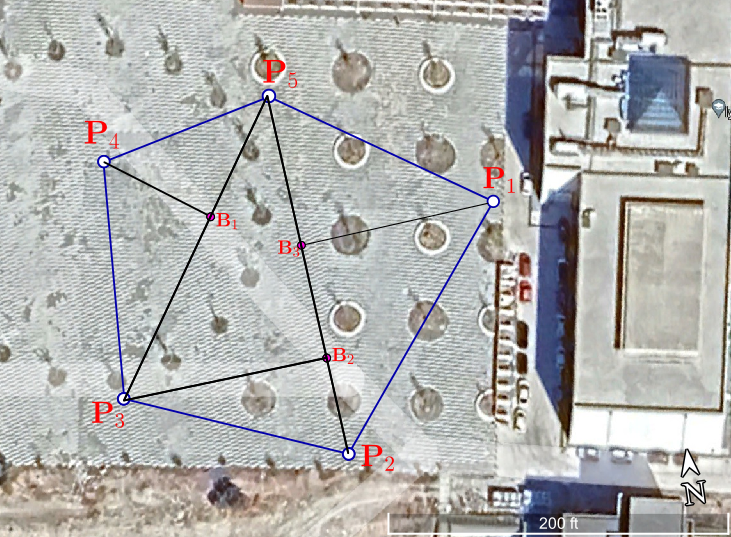
\includegraphics[width=0.8\linewidth]{a.png}
\end{figure}


\[
\begin{aligned}
&\begin{array}{l|l|l|l}
\hline P_3-P_5 & 70.17 & 69.70 & 69.20 \\
\hline P_5-P_3 & 68.27 & 69.40 & 70.56 \\
\hline P_3-P_5 & 20.40 & 67.50 & 69.80 \\
\hline P_2-P_5 & 69.21 & 67.40 & 66.48 \\
\hline P_5-P_2 & 67.18 & 66.93 & 64.85 \\
\hline P_2-P_5 & 66.22 & 67.841 & 69.41 \\
\hline P_1-B_3 & 33.64 & 30.70 & 20.69 \\
\hline P_4-B_1 & 21.32 & 26.30 & 27.753 \\
\hline P_3-B_2 & 40.33 & 50.79 & 52.78 \\
\hline
\end{array}
\end{aligned}
\]



\section*{Results}
\addcontentsline{toc}{section}{Results}

\begin{table}[ht!]
\caption{}
    \centering
    \begin{tabular}{lrlr}
    \toprule
     Side   &   MPV (m) & SD (m) &   SEM (m) \\
    \midrule
     P3-P5  &   63.8889 & 16.3354 &  5.445  \\
     P2-P5  &   67.2801 & 1.4314 &  0.4771 \\
     P1-B3  &   28.3433 & 6.7890  &  3.9196  \\
     P4-B1  &   25.1243 & 3.3737   &  1.9478  \\
     P3-B2  &   47.9667 & 6.6879  &  3.8613 \\
    \bottomrule
    \end{tabular}

\end{table}



\begin{table}[h!]
\centering
\caption{Calculated Areas of Triangles}
\label{tab:triangle_areas}
\begin{tabular}{@{}lc@{}}
\toprule
Triangle & Area (\(\operatorname{m}^2\)) \\ \midrule
Triangle 1 $(P_5P_3-P_4B_1)$ & 802.58 \\
Triangle 2 $(P_5P_2-P_1B_3)$ & 953.47 \\
Triangle 3 $(P_5P_2-P_3B_2)$ & 1613.60 \\ \bottomrule
\end{tabular}
\end{table}

\newpage
\section*{Discussion}
\addcontentsline{toc}{section}{Discussion}


In the discussion part, the results of the field practice on using geographic methods to figure out the area of a given pentagonal area are analysed and added to what is already known. The sides of a pentagon were carefully measured in this study using normal measuring tools and methods, such as Heron's formula for figuring out area. The method of measuring over and over, three times for each edge, helped reduce the chance of measurement mistakes, as shown by the low standard deviation seen for each edge. Sticking to strict methods made sure that the results were very accurate, showing that old-fashioned mapping methods still work in today's world of topographic analysis.

The estimated 95\% confidence range for the results is very close to the numbers that were found, which means that the data is very reliable and correct. According to this result, standard measuring methods, like using tape and Heron's formula, are very good at getting accurate area readings on flat ground. The study's results also add to the current discussion about whether and how traditional measuring methods are still useful in modern civil engineering and geography.

Nevertheless, it is important to note that the study has some problems. Even with repeated readings, using hand measurements adds a range of error that can be caused by human factors. Digital measuring technologies could be used in future studies to improve measurement accuracy and speed even more. Adding more problems related to topography, like rough ground and bigger areas, to the study would also help us learn more about how these standard mapping methods can be used in real life and what their limits are.

In the end, this field practice not only showed that traditional measuring methods are accurate and reliable for finding the area of complicated geometric shapes, but it also showed how important scientific rigour is for making sure measurements are correct. The results are useful for the study of geography because they show that traditional methods are still useful even though new technologies are coming out all the time. More study needs to be done on how to combine these old-fashioned methods with new technology in order to make geographic readings and studies more accurate and time-effective.

\section*{Conclusion}
\addcontentsline{toc}{section}{Conclusion}

Finally, this thorough investigation of the approaches used to determine the size of a pentagonal region using conventional surveying methods has shown their continued usefulness and accuracy in topography. The use of precise measuring techniques, such as taping and Heron's formula, has shown that the results are very accurate and that the scientific method of topographical surveying is based on rigorous principles of methodology.



\section*{Appendix}
\addcontentsline{toc}{section}{Appendix}

\begin{lstlisting}[language=Python]
import numpy as np
from scipy.stats import sem

measurements = {
    'P3-P5': [70.17, 69.70, 69.20, 68.27, 69.40, 70.56, 20.40, 67.50, 69.80],
    'P2-P5': [69.21, 67.40, 66.48, 67.18, 66.93, 64.85, 66.22, 67.841, 69.41],
    'P1-B3': [33.64, 30.70, 20.69],
    'P4-B1': [21.32, 26.30, 27.753],
    'P3-B2': [40.33, 50.79, 52.78],
}

def calculate_statistics(data):
    mpv = np.mean(data)
    sd = np.std(data, ddof=1)
    sem_val = sem(data, ddof=1)
    return mpv, sd, sem_val

results = []

for side, data in measurements.items():
    mpv, sd, sem_val = calculate_statistics(data)
    results.append([side, mpv, sd, sem_val])

distances = [result[1] for result in results]
sds = [result[2] for result in results]

total_distance = np.sum(distances)
propagated_error = np.sqrt(np.sum(np.array(sds) ** 2))

results.append(["Total", total_distance, "-", propagated_error])

from tabulate import tabulate
headers = ["Side", "MPV (m)", "SD (m)", "SEM (m)"]
table = tabulate(results, headers=headers, tablefmt="latex_booktabs")
print(table)


# Assumed MPV values for the sides
mpv_values = {
    'P5P3': 63.8889,  # Example MPV for P5P3
    'P4B1': 25.1243,  # Example MPV for P4B1
    'P5P2': 67.2801,  # Example MPV for P5P2
    'P1B3': 28.3433,  # Example MPV for P1B3
    'P3B2': 47.9667   # Example MPV for P3B2
}

areas = {    'Triangle1 (P5P3-P4B1)': 0.5 * mpv_values['P5P3'] * mpv_values['P4B1'],
    'Triangle2 (P5P2-P1B3)': 0.5 * mpv_values['P5P2'] * mpv_values['P1B3'],
    'Triangle3 (P5P2-P3B2)': 0.5 * mpv_values['P5P2'] * mpv_values['P3B2']
}

for triangle, area in areas.items():
    print(f"Area of {triangle}: {area:.2f} square units")

\end{lstlisting}
\end{document}